\documentclass[diploma]{BMSTU-IU8}

\student{И. И. Иванов}
\theme{Создание отчёта \\ по НИРС \\ или ВКР}
\group{ИУ8-999}

\supervisor{П. П. Петров}
\researchConsultant{П. П. Петров}
\designConsultant{П. П. Петров}
\technologicalConsultant{П. П. Петров}
\economicsConsultant{П. П. Петров}
\lawsConsultant{П. П. Петров}
\normController{П. П. Петров}

% \theme{Тест \hfill} % Тема для НИРСа заполняется по-другому
\studentFullName{Иванов Иван Иванович}
\profile{10У101}
\speciality{10.05.01 <<Компьютерная безопасность>>}
\specialization{10.05.01\_01 <<Математические методы защиты информации>>}
\supervisorWithDegree{доцент, к.т.н. Иванов И. И.}

% \newacronym{bd}{БД}{База данных.}
\newacronym{subd}{СУБД}{Система управления базами данных.}
\newacronym{ddl}{DDL}{Data Definition Language.}
\newacronym{dql}{DQL}{Data Query Language.}
\newacronym{dml}{DML}{Data Manipulation Language.}
\newacronym{dcl}{DCL}{Data Control Language.}
\newacronym{lsn}{LSN}{Log sequence number.}
\newacronym{id}{ID}{Identifier.}
\newacronym{uuid}{UUID}{Universally unique identifier.}


\newglossaryentry{id1}{
    name={База данных (БД)},
    description={это организованная коллекция данных, которая структурирована таким образом, чтобы данные можно было легко хранить, управлять, изменять и извлекать.},
}

\newglossaryentry{id7}{
    name={Бакет},
    description={это логический контейнер, в который помещаются данные для
    распределения по шардам (физическим серверам или узлам). Это абстракция,
    которая связывает ключ шардирования с конкретным шардом.}
}

\newglossaryentry{id6}{
    name={Кластер},
    description={это совокупность нескольких репликасетов, каждый из которых чаще всего хранит разный набор данных.}
}

\newglossaryentry{id11}{
    name={Ребалансировка},
    description={процесс перевозки бакетов с одного шарда на другой.}
}

\newglossaryentry{id5}{
    name={Репликасет (replicaset, набор реплик, шард)},
    description={это группа узлов, работающих в режиме репликации и объединенных для обеспечения отказоустойчивости и доступности данных.}
}

\newglossaryentry{id2}{
    name={Система управления базами данных (СУБД)},
    description={это программное обеспечение, предназначенное для создания, управления и обеспечения доступа к базам данных. Оно позволяет пользователям определять, создавать, изменять и управлять базой данных, а также обеспечивает взаимодействие между пользователями и базой данных через запросы и команды. Основные функции включают хранение, поиск, обновление и удаление данных, а также обеспечение целостности, безопасности и управления доступом к данным.}
}

\newglossaryentry{id4}{
    name={Спейс (space)},
    description={это основная логическая единица хранения данных Tarantool, аналогичная таблице в традиционных реляционных базах данных. Спейс содержит набор записей, каждая из которых называется кортежем (tuple). Структура спейса определяется схемой, которая включает количество и типы полей в кортежах, а также индексы для быстрого доступа к данным.}
}

\newglossaryentry{id10}{
    name={Шардирование},
    description={это принцип проектирования базы данных, при котором данные
    разбиваются на части и размещаются на разных наборах реплик (репликасеты,
    шарды).}
}

\newglossaryentry{id8}{
    name={LSN},
    description={это монотонно возрастающий идентификатор записи.}
}

\newglossaryentry{id9}{
    name={Vclock},
    description={это массив LSN, идентификаторами в котором являются ID узлов. Vclock представляет собой набор логических счетчиков для каждого узла в кластере, позволяя определить, какие изменения были применены на конкретном узле и какие еще предстоит синхронизировать.}
}

\addbibresource{main.bib}

\begin{document}
    % \maketitle
    \setcounter{page}{3} % Устанавливает счётчик страниц

    \structure{РЕФЕРАТ}

Алгоритм Шора серьёзно поставил под вопрос безопасность информации, основанную
на криптосистемах с открытым ключом. Однако для взлома широко используемой
схемы RSA-2048 требуются миллионы физических кубитов, что значительно превышает
текущие технические возможности. Здесь мы сообщаем об универсальном квантовом
алгоритме факторизации целых чисел, объединяющем классическую редукцию базиса
решетки с квантовым алгоритмом приближённой оптимизации (QAOA). Количество
требуемых кубитов равно $O(\log N / \log\log N)$, что сублинейно относительно
битовой длины целого числа $N$, делая этот алгоритм самым экономичным по числу
кубитов алгоритмом факторизации на сегодняшний день. Мы экспериментально
демонстрируем алгоритм, факторизуя целые числа размером до 48 бит с помощью 10
сверхпроводящих кубитов, что является наибольшим целым числом, факторизованным
на квантовом устройстве. Мы оцениваем, что квантовая схема с 372 физическими
кубитами и глубиной в тысячи операций необходима для того, чтобы бросить вызов
RSA-2048 при помощи нашего алгоритма. Наше исследование демонстрирует
значительные перспективы для ускорения применения текущих шумных квантовых
компьютеров и прокладывает путь к факторизации больших целых чисел, имеющих
реальное криптографическое значение.
 % Реферат

    \tableofcontents % Содержание
    \termsanddefenitions % Термины и определения
    % \listofabbreviations % Перечень сокращений и обозначений

    \structure{ВВЕДЕНИЕ}

Квантовые вычисления вступили в эпоху шумных квантовых устройств промежуточного
масштаба (NISQ) \cite{cite_1, cite_2}. Важной задачей эпохи NISQ является
демонстрация того, что устройства NISQ могут превзойти классические компьютеры
при решении задач с практической значимостью, то есть достижение практического
квантового преимущества. Алгоритмы, требующие минимальных ресурсов и
использующие ограниченное число доступных кубитов и глубину схем для решения
задач, сложных для классических вычислений, имеют особую важность. Вариационные
квантовые алгоритмы, использующие гибридную схему вычислений
«классика+квантовые вычисления», обладают значительным потенциалом для
получения значимого квантового преимущества в эпоху NISQ \cite{cite_3, cite_4,
cite_2, cite_5, cite_6}. Одним из таких алгоритмов является квантовый алгоритм
приближённой оптимизации (QAOA) \cite{cite_5}, первоначально предложенный для
решения задач на собственные значения, который впоследствии широко применялся в
различных областях, таких как химическое моделирование \cite{cite_7, cite_8},
машинное обучение \cite{cite_9}, а также инженерные приложения \cite{cite_10,
cite_11}.

Факторизация целых чисел является одной из важнейших основ современной
информационной безопасности \cite{cite_12}. Экспоненциальное ускорение
факторизации алгоритмом Шора \cite{cite_13} является выдающимся примером
превосходства квантовых вычислений. Однако выполнение алгоритма Шора на
отказоустойчивом квантовом компьютере требует значительных ресурсов
\cite{cite_14, cite_15}. На сегодняшний день наибольшее целое число,
факторизованное алгоритмом Шора на существующих квантовых системах, это число
21 \cite{cite_16, cite_17, cite_18}. Альтернативно, факторизация целых чисел
может быть сведена к задаче оптимизации, решаемой посредством адиабатических
квантовых вычислений (AQC) \cite{cite_19, cite_20, cite_21, cite_22} или QAOA
\cite{cite_23}. Более крупные числа были факторизованы этими методами на
различных физических системах \cite{cite_24, cite_25, cite_26, cite_27}.
Максимальные числа, факторизованные на данный момент, включают 291311 (19 бит)
в системе NMR \cite{cite_26}, 249919 (18 бит) на квантовом отжигателе D-Wave
\cite{cite_25}, 1099551473989 (41 бит) на сверхпроводящем устройстве
\cite{cite_27}. Однако следует отметить, что некоторые из факторизованных чисел
были специально подобраны с особыми структурами \cite{cite_28}, поэтому
наибольшее число, факторизованное универсальным методом на реальной физической
системе, на сегодняшний день составляет 249919 (18 бит).

В данной работе мы предлагаем универсальный квантовый алгоритм факторизации
целых чисел, требующий лишь сублинейные квантовые ресурсы. Алгоритм основан на
классическом алгоритме Шнорра \cite{cite_29, cite_30}, использующем редукцию
базиса решётки для факторизации целых чисел. Мы используем QAOA для оптимизации
наиболее трудоёмкой части алгоритма Шнорра, что ускоряет общее время
факторизации. Для целого числа $N$, имеющего $m$ бит, количество требуемых
кубитов в нашем алгоритме составляет $O(m / \log m)$, что сублинейно
относительно битовой длины числа $N$. Это делает наш алгоритм наиболее
экономным по числу кубитов по сравнению с существующими алгоритмами, включая
алгоритм Шора. С использованием данного алгоритма нами успешно факторизованы
числа 1961 (11 бит), 48567227 (26 бит) и 261980999226229 (48 бит) с
использованием, соответственно, 3, 5 и 10 кубитов на сверхпроводящем квантовом
процессоре. Число в 48 бит (261980999226229) также является наибольшим целым
числом, факторизованным универсальным методом на реальном квантовом устройстве.
Далее мы оцениваем квантовые ресурсы, необходимые для факторизации RSA-2048.
Согласно нашим расчётам, квантовая схема с 372 физическими кубитами и глубиной
порядка тысяч операций необходима для факторизации RSA-2048 даже в самой
простой одномерной системе. Подобный масштаб квантовых ресурсов, вероятно,
станет достижимым на устройствах NISQ в ближайшем будущем.

 % Введение

    \structure{ОСНОВНАЯ~ЧАСТЬ}

\section{Характеристика организации}

ВK Цифровые Технологии – подразделение VK, развивающее продукты и сервисы для
цифрового бизнеса. В основе экосистемы решений VK Цифровые технологии лежит
многолетний опыт развития интернет-сервисов и технологии на базе открытого
кода. VK Цифровые Технологии предоставляет готовые сервисы для решения бизнес
задач любой сложности, занимается заказной разработкой и управлением
ИТ-инфраструктурой на аутсорсе \cite{VkTech}.

В портфеле VK цифровые Технологии — облачные сервисы VK Cloud Solutions,
платформа in-memory вычислений Tarantool, платформа взаимодействия бизнеса и
государства VK Tax Monitoring, а также линейка программных продуктов для
управления персоналом, автоматизации производства и бизнес-процессов.

Tarantool как продукт появился 4 апреля 2016 года, когда Mail.ru Group (на
данный момент известная как VK) сообщила о создании нового направления бизнеса,
в рамках которого компания начала предоставлять корпоративным клиентам услуги в
области хранения данных.

Изначально Tarantool применялся только в собственных проектах Mail.ru, в том
числе в почтовом сервисе и облачном хранилище «Облако Mail.Ru». Затем компания
превратила эту СУБД в продукт с открытым исходным кодом, который к началу
апреля 2016 года внедрен рядом российских и международных компаний. В
частности, Tarantool начал использоваться сервисом бесплатных объявлений Avito,
социальной сетью знакомств Badoo и разработчиком систем информационной
безопасности Wallarm.

На сегодняшний день Tarantool активно используется в банковской сфере (среди
клиентов Tarantool можно выделить ВТБ, Альфа Банк, Банк Открытие и Газпромбанк)
и для ретейла и e-commerce (Магнит, Wildberries, Ситилинк, X5Group)
\cite{Tarantool}.

    \section{Шардирование}

В данном разделе рассматриваются фундаментальные аспекты шардирования как
ключевого метода горизонтального масштабирования баз данных. Исследуются
базовые принципы распределения данных, проводится сравнительный анализ
вертикального и горизонтального шардирования с практическими примерами их
применения. Особое внимание уделяется системному анализу преимуществ и
ограничений шардированной архитектуры. Завершает раздел обзор основных методов
шардирования с характеристикой их специфических особенностей и областей
эффективного применения.

\subsection{Общая информация}

Шардирование — это подход к организации баз данных, при котором массив данных
делится на части и распределяется по различным наборам реплик (шардам). Шард
является самостоятельным компонентом кластера и для повышения надёжности часто
включает не только мастера, но и реплики — серверы, хранящие копию данных
мастера.

Данная технология становится востребованной, когда система исчерпывает
возможности вертикального масштабирования (усиления мощности одного сервера) и
для дальнейшего роста ей требуется горизонтальное масштабирование (добавление
новых машин).

Популярные онлайн-сервисы со временем неизбежно нуждаются в масштабировании для
увеличения пропускной способности и быстродействия. Когда, например, социальная
сеть разрастается до многомиллионной аудитории, её работа на одном сервере
становится невозможной. Для безопасного и целостного распределения информации
между несколькими серверами применяется шардированная база данных.

\subsection{Виды шардирования}

Выделяют два вида шардирования:

\begin{itemize}
    \item Вертикальное — это вид шардирования, при котором
    данные распределяются по столбцам. Каждый шард в этой схеме хранит
    определенный набор колонок со всеми соответствующими строками. Данный
    подход особенно эффективен в сценариях, когда отдельные столбцы
    запрашиваются значительно чаще остальных.

    В качестве иллюстрации можно рассмотреть базу данных интернет-магазина,
    содержащую обширную информацию о товарах и клиентах. Для повышения
    производительности её можно разделить на два шарда: первый будет
    специализироваться на данных о покупателях, а второй — на информации о
    продуктах. Это позволит системе загружать только те столбцы, которые
    необходимы для выполнения конкретного запроса, оптимизируя таким образом
    использование ресурсов. Пример архитектуры вертикального шардирования
    представлен на рисунке~\ref{fig:fig01}.

\begin{figure}
  \centering
  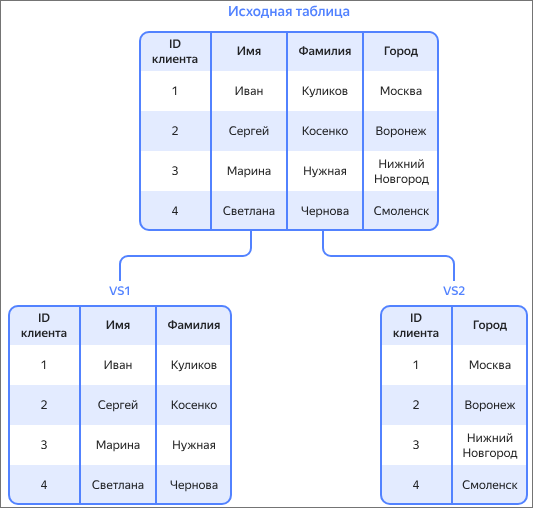
\includegraphics[scale=0.5]{inc/vertical-sharding.png}
  \caption{Вертикальное шардирование}
  \label{fig:fig01}
\end{figure}
    \item Горизонтальное — это вид шардирования, основанный на разделении строк
    таблицы в соответствии с определёнными правилами или ключами. При таком
    подходе каждый шард обладает идентичной схемой столбцов, но содержит
    уникальные наборы записей. Данная технология обеспечивает эффективное
    распределение операций чтения и записи между несколькими независимыми
    серверами, повышая общую производительность и отказоустойчивость системы.

    В качестве практического примера можно рассмотреть базу пользователей
    социальной сети. Для снижения нагрузки на инфраструктуру разработчики
    применяют горизонтальное партиционирование, используя хеш-функцию от
    первичного ключа (например, ID пользователя) для определения целевого шарда
    для каждой новой записи. Этот подход гарантирует равномерное распределение
    данных и запросов по всем узлам кластера. Пример реализации горизонтального
    шардирования демонстрируется на рисунке~\ref{fig:fig02}.

\begin{figure}
  \centering
  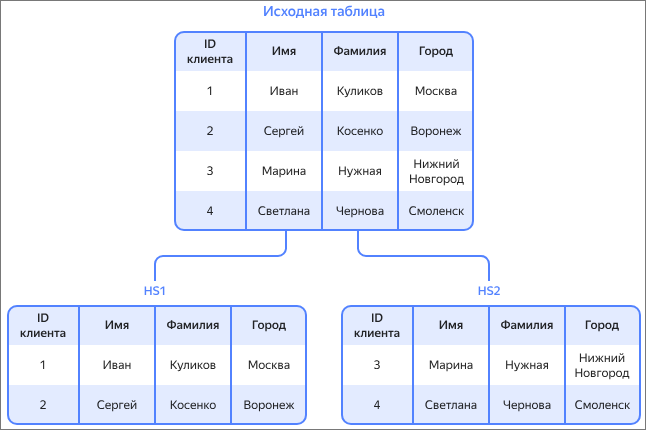
\includegraphics[scale=0.5]{inc/horizontal-sharding.png}
  \caption{Горизонтальное шардирование}
  \label{fig:fig02}
\end{figure}
\end{itemize}

\subsection{Преимущества и недостатки шардирования}

Когда монолитная база данных достигает пределов вертикального масштабирования,
шардирование становится эффективным решением для дальнейшего роста. Данная
архитектура предоставляет следующие преимущества:

\begin{itemize}
    \item \textbf{Преодоление аппаратных ограничений}. Популярные сервисы часто
    упираются в физические лимиты оборудования. Шардирование позволяет
    распределить информацию среди нескольких серверов, обеспечивая тем самым
    горизонтальное масштабирование и возможность практически неограниченного
    расширения.

    \item \textbf{Повышение отказоустойчивости}. Поскольку шарды физически
    размещаются на разных серверах, выход из строя одного из них не приводит к
    полному отказу системы. Это означает, что вместо полной недоступности
    сервиса может перестать функционировать лишь его некоторая часть, что
    значительно повышает надежность.

    \item \textbf{Увеличение производительности}. Монолитные базы данных часто
    страдают от конкуренции запросов, что снижает общую скорость работы.
    Шардирование распределяет нагрузку между узлами, что позволяет увеличить
    пропускную способность системы и ускорить обработку данных.
\end{itemize}

Несмотря на свою мощь, шардированная архитектура имеет ряд существенных
недостатков, которые делают её применение целесообразным не во всех ситуациях.

\begin{itemize}
    \item \textbf{Высокая сложность внедрения и сопровождения}. Процесс
    шардирования критически важен, и ошибки на этапе проектирования могут
    привести к потере или повреждению данных. Кроме того, разработка
    усложняется, так как исчезает единая точка входа для работы с данными, и
    команде приходится оперировать множеством изолированных сегментов.

    \item \textbf{Риск несбалансированной нагрузки}. Распределение данных может
    оказаться неравномерным, если критерии шардирования выбраны неудачно.
    Это приводит к ситуации, когда один шард (например, с данными популярных
    пользователей) обрабатывает большую часть запросов, создавая «горячую
    точку». Для устранения такой несбалансированности часто требуется
    трудоемкая процедура изменения шардирования, часто сопровождающаяся простоем.

    \item \textbf{Снижение эффективности сложных запросов}. Операции, которые
    требуют агрегации данных из нескольких шардов (например, JOIN'ы),
    выполняются значительно медленнее из-за необходимости сетевого
    взаимодействия с разными серверами и последующего объединения результатов.
    Это делает такие запросы более ресурсоемкими по сравнению с выполнением в
    рамках единой базы данных.
\end{itemize}

\subsection{Методы шардирования данных}

В практике распределённых баз данных применяются различные подходы к
шардированию, каждый из которых обладает специфическими характеристиками. Выбор
оптимальной стратегии зависит от конкретных требований и архитектурных
особенностей системы. Наиболее распространённые методы включают:

\begin{itemize}
    \item \textbf{Хеш-шардирование} — распределение данных между шардами
    осуществляется на основе вычисленного хеш-значения от ключа записи. Данный
    метод обеспечивает равномерное распределение нагрузки и высокую доступность
    системы, но осложняет выполнение запросов по диапазонам значений.

    \item \textbf{Диапазонное шардирование} — разделение данных производится
    согласно заданным интервалам значений ключевых атрибутов. Подход отличается
    простотой реализации и эффективностью при выполнении запросов в пределах
    определённого диапазона, однако может приводить к неравномерному
    распределению нагрузки между шардами.

    \item \textbf{Круговое шардирование} — шарды организуются в логическое
    кольцо, где каждый узел отвечает за определенный сегмент данных. Запросы
    маршрутизируются в соответствии с позицией шарда в кольцевой структуре.
    Метод обеспечивает равномерное распределение запросов, но требует сложной
    процедуры перераспределения данных при изменении количества шардов.

    \item \textbf{Динамическое шардирование} — система автоматически адаптирует
    структуру хранения в зависимости от текущей нагрузки и объема данных.
    Несмотря на высокую гибкость и масштабируемость, данный подход требует
    сложной системы мониторинга, балансировки нагрузки и тщательно продуманной
    архитектуры.
\end{itemize}


    \section{Обзор шардирования в СУБД Tarantool}

В этом разделе детально исследуется реализация механизма шардирования в СУБД
Tarantool. Кроме того, анализируются ключевые компоненты модуля шардирования,
понимание которых необходимо для реализации предложенного подхода к выполнению
Map запросов на репликах.

\subsection{Обзор}

В Tarantool логически связанные узлы, работающие с идентичными копиями базы
данных, объединяются в репликасеты (replicaset). В рамках каждого набора узлам
назначаются роли: мастер (master) или реплика (replica). Обработка запросов
на изменение данных (DDL, DML, DCL) осуществляется исключительно на мастере,
тогда как реплики обслуживают только запросы на чтение (DQL). Между узлами
внутри репликасета поддерживается процесс синхронизации данных посредством
репликации.

Реализация шардирования в Tarantool обеспечивается модулем \textit{vshard}
\cite{VshardGithub}, разработанным на языке Lua. Этот выбор обусловлен тем, что
Tarantool сочетает функциональность СУБД с возможностью исполнения прикладной
логики, которая реализуется на Lua.

Модуль \textit{vshard} в Tarantool обеспечивает распределение кортежей набора
данных среди нескольких шардов, представляющх собой репликасеты. Каждый шард
обрабатывает только определённое подмножество общих данных, что позволяет
масштабировать систему под повышенную нагрузку путём добавления новых шардов.

Модуль \textit{vshard} предоставляет API маршрутизатора (router) и
API хранилища (storage) для разработки приложений, поддерживающих
шардирование.

\subsection{Архитектура шардированного кластера Tarantool}

Рассмотрим распределенный кластер Tarantool, состоящий из подкластеров,
называемых шардами, каждый из которых хранит некоторую часть данных. Каждый
шард, в свою очередь, представляет собой набор реплик (replica set), состоящий
из нескольких реплик, одна из которых служит главным узлом (master node),
обрабатывающим все запросы на чтение и запись.

Весь набор данных логически разделен на заранее определенное количество
виртуальных бакетов (далее - бакеты), каждому из которых присвоен уникальный
номер в диапазоне от 1 до N, где N - общее количество бакетов. Количество
бакетов специально выбирается на несколько порядков больше потенциального
количества узлов кластера, даже с учетом будущего масштабирования кластера.
Например, при M проектируемых узлах набор данных может быть разделен на 100M
или даже 1000M бакетов. При выборе количества бакетов следует соблюдать
осторожность: если оно слишком велико, это может потребовать дополнительной
памяти для хранения информации о маршрутизации; если слишком мало, это может
уменьшить детализацию перебалансировки.

Каждый шард хранит уникальное подмножество бакетов, что означает, что бакет не
может принадлежать нескольким шардам одновременно, как показано на
рис~\ref{fig:fig03}.

\begin{figure}
  \centering
  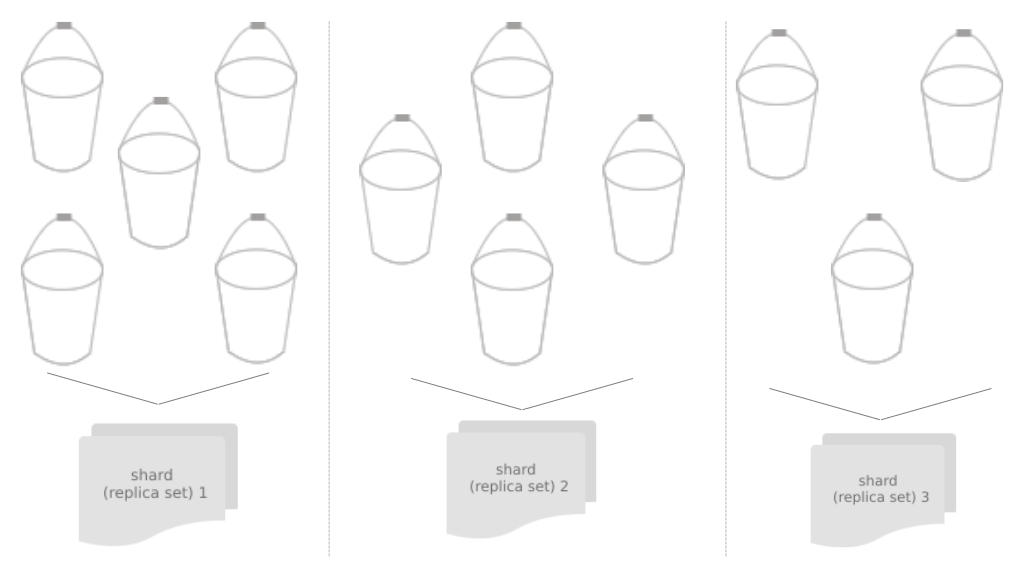
\includegraphics[scale=0.7]{inc/bucket.png}
    \caption{Виртуальные бакеты \cite{VshardDoc}}
  \label{fig:fig03}
\end{figure}

Данное соответствие шардов и бакетов хранится в таблице в одном из системных
спейсов Tarantool, причем каждый шард содержит только определенную часть этой
карты, которая покрывает те бакеты, которые были назначены данному шарду.

Помимо таблицы соответствия, идентификатор бакета также хранится в специальном
поле каждого кортежа каждой таблицы, участвующей в шардировании.

Когда шард получает любой запрос (кроме SELECT) от приложения, этот шард
проверяет идентификатор бакета, указанный в запросе, по таблице идентификаторов
бакетов, принадлежащих данному узлу. Если указанный идентификатор бакета
недействителен, запрос завершается со следующей ошибкой: "wrong bucket". В
противном случае запрос выполняется, и всем данным, созданным в процессе,
присваивается идентификатор бакета, указанный в запросе. Важно отметить, что
запрос должен изменять только те данные, которые имеют тот же идентификатор
бакета, что и сам запрос.

Хранение идентификаторов бакетов как в самих данных, так и в таблице
соответствия обеспечивает целостность данных независимо от логики приложения и
делает перебалансировку прозрачной для приложения. Хранение таблицы
соответствия в системном спейсе гарантирует согласованность шардирования в
случае отказа, поскольку все реплики в шарде разделяют общее состояние таблицы.

Шардированный кластер в Tarantool состоит из:

\begin{itemize}
    \item \textbf{Одного или нескольких наборов реплик}:
    \begin{itemize}
        \item Каждый набор реплик должен содержать как минимум два экземпляра
              хранилища (storage)
        \item Для обеспечения избыточности рекомендуется иметь 3 или более
              экземпляров хранилища в наборе реплик
    \end{itemize}

    \item \textbf{Одного или нескольких маршрутизаторов (router)}:
    \begin{itemize}
        \item Количество экземпляров маршрутизаторов не ограничено
        \item Его следует увеличивать, если существующие экземпляры
              маршрутизаторов становятся узким местом из-за нагрузки на ЦПУ или
              ввод-вывод
    \end{itemize}
    \item \textbf{Балансировщика (Rebalancer)}
\end{itemize}

Структура шардированного кластера представлена на рис~\ref{fig:fig04}

\begin{figure}
  \centering
  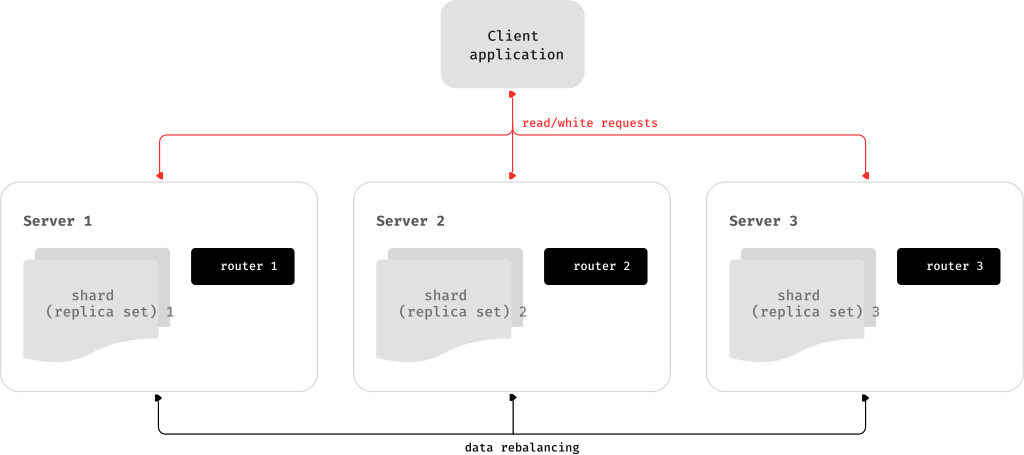
\includegraphics[scale=0.5]{inc/schema.png}
  \caption{Архитектура шардированного кластера \cite{VshardDoc}}
  \label{fig:fig04}
\end{figure}

\subsection{Маршрутизатор (router)}

Маршрутизатор (далее роутер) представляет собой автономный программный
компонент, который направляет запросы на чтение и запись от клиентского
приложения к соответствующим шардам.

Все запросы от приложения поступают в шардированный кластер через роутер.
Роутер обеспечивает прозрачность топологии шардированного кластера для
приложения, скрывая от него:

\begin{itemize}
\item количество и расположение шардов,
\item процесс перебалансировки данных,
\item факт и процесс отработки отказа при сбое реплики.
\end{itemize}

Роутер может самостоятельно вычислять идентификатор бакета при условии, что
приложение явно определяет правила вычисления идентификатора бакета на основе
данных запроса. Для этого роутер должен знать схему данных.

Роутер не имеет постоянного состояния и не хранит топологию кластера, а также
не выполняет балансировку данных. Это автономный программный компонент, который
может работать на уровне хранилища или на уровне приложения в зависимости от
особенностей приложения.

Роутер поддерживает постоянный пул соединений со всеми хранилищами, создаваемый
при запуске. Такой подход помогает избежать ошибок конфигурации. После создания
пула роутер кэширует текущее состояние спейса \texttt{\_bucket} для ускорения
маршрутизации. В случае перемещения идентификатора бакета на другое хранилище в
результате ребалансировки данных или при переходе одного из шардов на реплику,
роутер обновляет таблицу маршрутизации.

Шардирование не интегрировано в какую-либо централизованную систему хранения
конфигурации. Предполагается, что само приложение обрабатывает все
взаимодействия с такими системами и передает параметры шардирования. При этом
конфигурация может изменяться динамически - например, при добавлении или
удалении одного или нескольких шардов:

\begin{itemize}
\item Для добавления нового шарда в кластер системный администратор сначала
    изменяет конфигурацию всех роутеров, а затем конфигурацию всех хранилищ.
\item Новый шард становится доступным уровню хранилища для перебалансировки.
\item В результате перебалансировки один из виртуальных бакетов перемещается на
    новый шард.
\item При попытке доступа к виртуальному бакету роутер получает специальный код
    ошибки, указывающий новое местоположение бакета.
\end{itemize}

\subsection{Ребалансировщик}

Ралансировщик представляет собой фоновый процесс перебалансировки, который
обеспечивает равномерное распределение бакетов между шардами. В процессе
перебалансировки происходит миграция бакетов между наборами реплик.

Балансировщик периодически "просыпается" и перераспределяет данные из наиболее
загруженных узлов в менее загруженные узлы. Перебалансировка запускается, если
дисбаланс набора реплик превышает заданный в конфигурации пороговый уровень.

Дисбаланс набора реплик рассчитывается следующим образом:
\begin{equation}
|etalon\_bucket\_number - real\_bucket\_number| / etalon\_bucket\_number * 100
\end{equation}

\subsection{Миграция бакетов}

Набор реплик, с которого выполняется миграция бакета, называется
источником (source); целевой набор реплик, на который выполняется
миграция, называется приемником (destination).

Во время миграции бакет может находиться в различных состояниях:

\begin{itemize}
\item \texttt{ACTIVE} -- бакет доступен для запросов на чтение и запись.
\item \texttt{PINNED} -- бакет заблокирован для миграции на другой набор
    реплик. В остальном заблокированные бакеты аналогичны бакетам в состоянии
        ACTIVE.
\item \texttt{SENDING} -- бакет в настоящее время копируется на набор реплик
    приемник; запросы на чтение к набору реплик источник все еще
        обрабатываются.
\item \texttt{RECEIVING} -- бакет в настоящее время заполняется; все запросы к
    нему отклоняются.
\item \texttt{SENT} -- бакет был мигрирован на набор реплик приемник. Роутер
    использует состояние SENT для вычисления нового местоположения бакета.
        Бакет в состоянии SENT автоматически переходит в состояние GARBAGE
        через 0.5 секунды.
\item \texttt{GARBAGE} -- бакет уже был мигрирован на набор реплик приемник во
    время перебалансировки; или бакет изначально находился в состоянии
        RECEIVING, но во время миграции произошла ошибка. Бакеты в состоянии
        GARBAGE удаляются сборщиком мусора.
\end{itemize}

Процесс миграции бакетов представлен на рис~\ref{fig:fig05}. Она выполняется
следующим образом:

\begin{enumerate}
\item На целевом наборе реплик (destination) создается новый бакет, которому
    присваивается состояние \texttt{RECEIVING}, начинается копирование данных,
        и бакет отклоняет все запросы.
\item Бакету в исходном наборе реплик (source) присваивается состояние
    \texttt{SENDING}, и бакет продолжает обрабатывать запросы на чтение.
\item После завершения копирования данных бакет в исходном наборе реплик
    переводится в состояние \texttt{SENT} и начинает отклонять все запросы.
\item Бакет в целевом наборе реплик переводится в состояние \texttt{ACTIVE} и
    начинает принимать все запросы.
\end{enumerate}

\begin{figure}
  \centering
  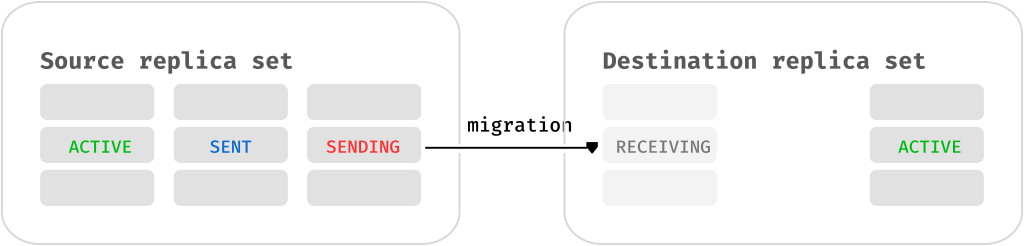
\includegraphics[scale=0.7]{inc/states.png}
  \caption{Пересылка бакета \cite{VshardDoc}}
  \label{fig:fig05}
\end{figure}

\subsection{Системный спейс \_bucket}

В системном спейсе \texttt{\_bucket} каждого набора реплик хранятся идентификаторы
бакетов, присутствующих в данном наборе реплик. Спейс содержит следующие поля:

\begin{itemize}
\item \texttt{bucket} -- идентификатор бакета
\item \texttt{status} -- состояние бакета
\item \texttt{destination} -- UUID целевого набора реплик
\end{itemize}

Пример вывода команды \texttt{\_bucket:select\{\}} представлен на рис
~\ref{fig:fig06}.

\begin{figure}
  \centering
  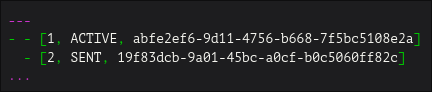
\includegraphics[scale=0.5]{inc/bucket-space.png}
  \caption{Содержание спейса \_bucket}
  \label{fig:fig06}
\end{figure}

После завершения миграции бакета в таблице заполняется поле UUID целевого
набора реплик. Пока бакет находится на исходном наборе реплик, значение UUID
целевого набора реплик равно NULL.

\subsection{Обработка запроса клиента}

Запросы к базе данных могут выполняться приложением или с использованием
хранимых процедур. В любом случае, идентификатор бакета должен быть явно указан
в запросе.

Все запросы сначала перенаправляются роутеру. Единственной операцией,
поддерживаемой роутером, является \texttt{call}. Данная операция выполняется с
помощью функции \texttt{vshard.router.call()}:

\begin{verbatim}
result = vshard.router.call(<bucket_id>, <mode>, <function_name>, \\
        {<argument_list>}, {<opts>})
\end{verbatim}

Обработка запросов выполняется следующим образом:

\begin{enumerate}
\item Роутер использует идентификатор бакета для поиска соответствующего набора
    реплик в таблице маршрутизации.
\item Если соответствие идентификатора бакета набору реплик неизвестно роутеру
    (fiber обнаружения еще не заполнил таблицу), роутер отправляет запросы ко
    всем хранилищам, чтобы определить местоположение бакета.
\item После обнаружения бакета шард проверяет:
\begin{itemize}
    \item наличие бакета в системном спейсе \texttt{\_bucket} набора реплик;
    \item находится ли бакет в состоянии \texttt{ACTIVE} или \texttt{PINNED}
        (для запросов на чтение также допустимо состояние \texttt{SENDING}).
\end{itemize}
\item Если все проверки успешны, запрос выполняется. В противном случае он
    завершается с ошибкой: "\texttt{WRONG\_BUCKET}".
\end{enumerate}

    \section{Дизайн-документ по реализации функционала Map по репликам}

\begin{itemize}
    \item Текущая реализация Map запроса по репликам у клиента ведет к
    дублированию, потере и повреждению данных;
    \item В vshard будут добавлены новые запросы: \texttt{map\_callro},
        \texttt{map\_callre}, \texttt{map\_callbro}, \texttt{map\_callbre};
    \item \texttt{map\_*} запросы (даже те, которые выполняются на репликах)
        замедляют ребалансировку. Пользователь может регулировать распределение
        между map запросами и перевозом бакетов с использованием опций
        sched\_ref\_quota, sched\_move\_quota.
\end{itemize}

\subsection{Мотивация}

В бизнес-логике клиента очень много map-запросов, однако \texttt{vshard} на
данный момент не предлагает никакого решения для совершения map-запросов по
репликам, вследствии чего клиент вынужден писать собственные решения с
использованием \texttt{vshard.router.routeall}, которые выполняются с рисками
нарушения консистентности и целостности получаемых данных (дублирование и
потеря).

Базово сейчас \texttt{map\_callro} у клиента выглядит так (еще есть логика на
пропуск репликасетов из \texttt{routeall} при определенных условиях):

\begin{verbatim}
for _, rs in pairs(vshard.router.routeall()) do
    rs:callbro('box.space.card:select()', nil, {timeout = <number>})
end
\end{verbatim}

Это крайне небезопасно:

\begin{enumerate}
\item \textbf{Дублирование данных} - бакет может находиться в процессе
    пересылки (\texttt{state = SENDING}) или уже даже быть послан
        (\texttt{state = SENT}). Данные не удаляются во время пересылки, только
        после ее полного окончания, поэтому когда бакет переезжает данные есть
        на двух шардах. При \texttt{select} по спейсу получим дублирование
        данных. Даже если бакет полностью переехал, дублирование возможно:
        пришли на первый репликасет, там данные еще есть, пока идем до второго,
        они переехали, пришли на второй, там эти же данные уже есть. Если бакет
        в процессе удаления, то можно прочитать часть бакета, а полностью он
        будет только там, куда уехал, снова дублирование.

\item \textbf{Потеря данных} - мы идем на первый репликасет, данных там пока
    нет, нам вернули результат. Пока идем до следующего, он успевает переслать
        бакет на первый репликасет (полностью переслать, с удалением данных).
        Мы дошли до него, данных там тоже не будет. Map-запрос потерял данные.

\item \textbf{"Повреждение данных"} - можно прочитать неконсистентное состояние
    данных (\texttt{state = GARBAGE}). Допустим пользователь добавлял в один
        бакет в одной транзакции таплы 1, 2, 3, 4, 5. Бакет уехал. Таплы 1, 2,
        3 уже удалились. Таплы 4 и 5 еще нет. Запрос их прочитает, т.е.
        половину пользовательской транзакции.

\end{enumerate}

\texttt{Vshard}-у следует предоставить собственное решение для выполнения
map-запроса по репликам, который не будет дублировать и терять бакеты.

\subsection{Текущая работа Map запроса по мастерам (map\_callrw)}

\texttt{vshard.router.map\_callrw} принимает в качестве аргумента функцию,
которая вызывается на мастерах в кластере с гарантией, что в случае успешного
выполнения она была выполнена при доступности всех бакетов для чтения и записи.
Под консистентностью в рамках Map-Reduce понимается, что все данные были
доступны и не перемещались в процессе выполнения запросов Map. Чтобы сохранить
консистентность, добавлена третья стадия - Ref. Таким образом, алгоритм на
самом деле называется Ref-Map-Reduce.

Ref-ы отправляются до этапа Map, чтобы закрепить бакеты на репликасетах и
гарантировать, что они не будут перемещаться до завершения стадии Map. Если
хотя бы один Ref не удалось проставить, то пользователю возвращается ошибка.

Если все Ref-ы успешно завершены, начинается рассылка запросов Map. Эти запросы
выполняют пользовательскую функцию и после удаляют Ref-ы, чтобы снова разрешить
ребалансировку. Рассылка запросов Map производится параллельно, ко всем
необходимым мастерам.

На уровне стораджей существуют дополнительные механизмы, чтобы гарантировать,
что Map-Reduce не блокирует ребалансировку навсегда и наоборот: что
ребалансировка не заблокирует полностью Map-Reduce. Это конкурирующие процессы.
В vshard есть опции: \texttt{sched\_ref\_quota}, \texttt{sched\_move\_quota}.
Если \texttt{move\_quota = 2} и \texttt{ref\_quota = 15}, то это означает, что
максимум 2 бакета могут переехать, если есть запросы на ref. И наоборот,
максимум 15 рефов может быть сделано, если нужно перевозить бакет.

Подробней про работу \texttt{map\_callrw} можно прочитать в дизайн-документе
соответсвующем дизайн-документе \cite{MapCallrwRfc}.

Аргументы vshard.router.map\_callrw:

\begin{itemize}
\item \texttt{func}: Имя вызываемой функции.
\item \texttt{args}: Аргументы функции, переданные в формате netbox (в виде
    массива).
\item \texttt{opts.timeout}: Таймаут в секундах. Учтите, что Ref-ы могут
    оставаться на хранилищах в течение всего этого таймаута, если что-то пойдет
        не так, например, возникнут сетевые проблемы. Поэтому лучше не
        использовать значение больше, чем необходимо.
\item \texttt{opts.return\_raw}: true/false. Если указано, возвращаемые
    значения не декодируются в нативные объекты Lua и остаются упакованными как
        объект msgpack (см. модуль msgpack). По умолчанию все значения
        декодируются. Это может быть нежелательно, если возвращаемые значения
        будут сразу пересылаться по сети.
\item \texttt{opts.bucket\_ids}: Массив ID бакетов, которые должны быть
    охвачены Map-Reduce. Если она указана, Map-Reduce выполняется только на
        мастерах, содержащих хотя бы один из этих бакетов. В противном случае
        Map-Reduce выполняется на всех мастерах кластера.
\end{itemize}

\subsection{Дизайн}

В map-запросах все фазы Ref-Map выполняются на одной и той же реплике:

\begin{itemize}
\item \texttt{map\_callrw} -- выполняется только на мастере. Реализован в
    текущей версии.

\item \texttt{map\_callro} -- реплика выбирается на основе весов в конфигурации
    роутера (чем меньше вес, тем реплика приоритетнее). Такой репликой может
        являться и мастер (при использовании весов по умолчанию мастер является
        наиболее приоритетной репликой). Выбор реплики не является постоянным и
        может временно меняться, если самая приоритетная реплика недоступна.

\item \texttt{map\_callre} -- предпочтение отдается не мастеру (но все еще
    может быть выполнена на мастере как последняя мера, если все реплики не
        ответили).

\item \texttt{map\_callbro} -- round-robin балансировка по всем инстансам в
    репликасете, может быть как мастер, так и реплика.

\item \texttt{map\_callbre} -- round-robin балансировка, но с предпочтением
    пропускать мастера.
\end{itemize}

\subsubsection{Ref стадия запроса}

Для map запросов по репликам применяются те же рефы, что используются сейчас
для мастеров, ref полностью локальный (если инстанс не мастер, то запрос на
мастера не совершается). Реф происходит до запроса ко всем репликам, в
отдельную фазу, как и для \texttt{map\_callrw}. Ref так же как и в случае c
\texttt{map\_callrw} дожидается, чтобы все бакеты на инстансе были
\texttt{ACTIVE} или \texttt{PINNED}. Если не получается зарефать (идет
ребалансировка), возвращается ошибка, ни один map запрос не будет выполнен.
Если ref успешно создан на всех репликах, выполняется пользовательская функция,
после чего реф удаляется.

Ref блокирует все бакеты на инстансе, пока висит Ref, ребалансировка
невозможна.

\subsubsection{Map запросы и ребалансировка бакетов}

Мастеру приходит запрос на перевоз N бакетов. Он собирает эти N бакетов и перед
началом отправления делает \texttt{sched.move\_start} локально. В случае успеха
мастер переводит бакеты в состояние \texttt{SENDING}. Далее, данные не
отправляются/получаются, пока мы не получим на это разрешение всех реплик в
нашем репликасете. Мастер дожидается на каждой из реплик выполнение функции
\texttt{bucket\_move\_prepare\_replica(timeout, vclock\_of\_first\_bucket)}, где
\texttt{vclock} -- это vclock мастера после того, как был изменен статус
первого измененного бакета. Эта функция выполняется на реплике следующим
образом:

\begin{itemize}
\item Вызывает \texttt{sched.move\_start} чтобы создать конкуренцию за ресурсы
    на репликах и обеспечить заданное пользователем (с помощью
        \texttt{sched\_*\_quota} опций) распределение между перевозом бакетов и
        ref запросами.
\item Дожидается, чтобы реплика достигла необходимого vclock. Т.е. получила
    хотя бы один \texttt{SENDING} бакет. Этого достаточно, чтобы новые рефы не
        могли быть созданы и ждать, пока отреплицируются все, смысла ждать нет.
\item Вызывает \texttt{sched.move\_end(1)}. Отныне новые рефы не могут быть
    созданы, так как бакет перемещается.
\end{itemize}

Если хотя бы одна реплика ответила ошибкой, бакеты не будут посылаться, ошибка
отправления бакета. Не меняем состояние бакета, в случае ошибок этим занимается
recovery (не забыть разбудить в случае фейла) и gc. Если все реплики смогли
подтвердить перевоз бакетов, то обращаемся к мастеру, на который данные будут
отправляться: \texttt{bucket\_recv\_prepare\_master(timeout, buckets)}. Он
переводит бакеты в состояние \texttt{RECEIVING}, делает вызов по репликам
\texttt{bucket\_move\_prepare\_replica}, чтобы убедиться, что новые рефы не смогут
быть созданы и дождаться окончания \texttt{map\_callro}. Если успешно,
возвращает ок.

Вся работа мастера, описанная выше объединяется в функцию
\texttt{bucket\_send\_prepare\_master(timeout, buckets)}.

Таким образом на посылку/получение одного батча (откуда посылаем: батч - все
route, которые пришли, куда посылаем: батч - набор бакетов от конкретного
репликасета) нужно будет совершить только по одному запросу на каждую из
реплик. Дальше при пересылке бакетов работают воркеры, как обычно (но не
переводя в состояние \texttt{SENDING} и то, что описано выше).

Чтобы предотвратить одновременную посылку одного и того же бакета (например,
когда ребалансер пытается послать и пользователь вызывает
\texttt{bucket\_send}), \texttt{M.rebalancer\_transfering\_buckets[bid] =
'preparing'} выполняется для каждого из бакетов перед локальным
\texttt{sched\_move\_start} на мастере (в самом начале
\texttt{bucket\_send\_prepare\_master}). Затем когда воркер начинает работу он
проверяет, что статус бакета \texttt{preparing} (можно было бы добавить статус
\texttt{prepared} после того, как дождались разрешения реплик, но выглядит
бессмысленно, мы не должны отдавать работу в воркеры, если бакет не разрешили
пересылать), меняет его в \texttt{transfering}. На принимающей стороне
состояние бакета меняется на \texttt{preparing} в
\texttt{bucket\_recv\_prepare\_master} (recovery должен разруливать эти статусы
и подчищать их, если на отправляющей стороне
\texttt{rebalancer\_transfering\_buckets} в \texttt{nil}). На стадии
\texttt{bucket\_recv} состояние бакета меняется на \texttt{transfering}. По
умолчанию \texttt{M.rebalancer\_transfering\_buckets[bid] = nil}.

Если \texttt{bucket\_recv} видит, что бакета не существует, тогда он вызывает
\texttt{bucket\_move\_prepare\_replica}. Необходимо, чтобы ребалансинг работал,
если отправитель на старой версии, а получатель на новой. Если отправитель на
новой версии, то пересылка бакета будет падать на стадии
\texttt{bucket\_recv\_prepare\_master}.

\subsection{Последующе действия}

Описанное в данном пункте будет реализовано только по запросу от пользователей.
В изначальную имплементацию map запросов этот пункт не входит.

Во все \texttt{map\_*} запросы добавляется новая опция
\texttt{consistency\_coverage\_mode}. При обоих режимах выполняется попытка
остановить ребалансировку!

\begin{itemize}
    \item \texttt{consistency\_coverage\_mode = 'full'}. Запрос будет выполнен
        везде или не будет выполнен вовсе, запрос гарантированно будет без
        дублирования данных, без их потери, т.е. будет выполнен на каждом
        бакете и ровно один раз.

    \texttt{map\_*} запрос выполняется в две фазы: Ref - попытка приостановить
        ребалансировку на всех инстансах, Map - выполнение пользовательской
        функции. Необходим в первую очередь для \texttt{map\_callrw}. Если
        ошибка на стадии Ref - возврат ошибки пользователю, функция не будет
        исполнена нигде.

    \item \texttt{consistency\_coverage\_mode = 'accidental'}. Запрос будет
        выполнен там, где удастся остановить ребалансировку. Там, где он
        выполнится, дублирования данных не будет, т.е. функция не будет
        исполнена дважды на одном и том же бакете, "not more than once". Но
        данные в рамках кластера могут быть частично прочитаны и записаны, нет
        гарантии "at least once" для каждого из бакетов.

    \texttt{map\_*} запрос тоже выполняется в две фазы. Единственное отличие от
        \texttt{full} режима: если на стадии Ref не удалось выполнится на всех
        инстансах, то стадия Map выполняется на тех инстансах, где Ref прошел
        успешно. Всегда возвращается таблица типа \texttt{\{<replicaset\_uuid>
        = <returned\_value>, ...\}}.

    Полезен при \texttt{map\_*} запросах на чтение.
\end{itemize}

Первый режим необходим для работы \texttt{map\_callrw}. Необходимо
гарантировать, что запрос выполнен на всех репликасетах, а не на их части. Ибо
если мы записали что-то только на части репликасетов, то это беда, частичное
обновление данных. Однако, если пользователь, например, читает только с
мастеров (например, для обеспечения максимальной согласованности данных), то
имеет смысл использовать \texttt{accidental}.

Второй режим будет очень полезен для \texttt{map\_callro}, так как в
большинстве случаев лучше прочитать хоть что-то (например делаем select по
спейсу), чем не читать вообще ничего. Однако если данные невозможно
использовать частично, \texttt{consistency\_coverage\_mode} все равно должен
стоять в \texttt{full}.

Режим \texttt{full} существует уже сейчас в \texttt{map\_callrw}. Будет
добавлен только \texttt{accidental}. Для map запросов по репликам в изначальной
имплементации реализовываем только \texttt{full} режим, \texttt{accidental}
добавляется в тикет.

\subsection{Рассмотренные альтернативы}

\subsubsection*{Вызывать sched.move\_start на репликах перед изменением состояния бакета}

Была идея, чтобы перед отправлением/получением бакета, до изменения состояния
бакета совершать \texttt{sched.move\_start}. Только если сумели дождаться 0
рефов везде, можно начинать ребалансировку, производится перевод бакета в
нужное состояние на мастере, бакет перевозится. Реплика автоматически зовет
\texttt{sched.move\_end} в on\_replace триггере когда получает по репликации
\texttt{replace} в \texttt{\_bucket}. Если же где-то есть рефы и мы не смогли
дождаться, то отменяем все с помощью \texttt{sched.move\_end} с мастера.

Однако тут мы наблюдаем стандартную проблему 2PC. Если мы не используем
таймаут, после которого автоматически зовется \texttt{sched.move\_end}, то,
если мастер падает сразу после вызова \texttt{sched.move\_start}, реплика
навсегда заблокирована. Если мы используем таймауты, то можем получить
неконсистентные данные, так как таймаут может отработать раньше, чем придет
replace в \_bucket, будет создан ref для map\_call, а потом к нам долетит
replace: во время исполнения функции пользователя мы нарушили гарантии того,
что состояние бакетов не будет меняться.

\subsection*{При посылке бакета разрешать рефать реплику}

Была идея разрешить рефать реплики, пока бакет находится в состоянии
\texttt{SENDING}. Появляется новый тип глобального рефа (определенного в модуле
ref.lua): \texttt{ref.add\_ro}, старый переименовывается в
\texttt{ref.add\_rw}. В отличии от текущего rw ref-а он ждет, чтобы все бакеты
были читаемыми (т.е. \texttt{ACTIVE}, \texttt{PINNED}, или \texttt{SENDING}).
Именно этим глобальным рефом и пользуются реплики при map\_call.

В случае отправления бакета. Переводим бакет в состояние \texttt{SENDING},
начинаем отправлять. Читать \texttt{SENDING} бакеты можно. Он не будет удален,
пока существуют рефы на этот бакет, однако нужно заставить gc учитывать ro рефы
на стораджах. Поведение такое же, как для обычных call запросов: могут
существовать рефы, даже если бакет в состоянии \texttt{SENT}, \texttt{GARBAGE}.

В случае получения бакета (\texttt{RECEIVING}) рефать такой сторадж запрещено,
мастер дожидается 0 ro ref-ов после перевода бакета в состоянии
\texttt{RECEIVING}.

Тут проблема в том, что бакет может читаться в состоянии \texttt{SENT/GARBAGE}.
Начали выполнять map\_callro прям перед окончанием переезда, успели зарефать на
реплике, откуда посылалось (т.е. до перевода из \texttt{SENDING} в
\texttt{SENT}), пришли на тот, куда прислалось, когда там бакет уже в
\texttt{ACTIVE}, получим дублирование данных.

\subsection*{Включение map\_callro только по опции в конфигурации}

Предполагается, что \texttt{map\_call} с \texttt{mode = 'read'} будет
использоваться редко, а потому нет смысла усложнять ребалансинг бакетов для
пользователей, которые не пользуются данной функцией. Для этого добавляется
новая опция конфигурирования vshard (будет проброшена в cartridge):
\texttt{enable\_read\_map\_calls} (name subject to change) - опция может быть
задана на уровне репликасета или глобально в конфигурации (для всех
репликасетов сразу). Включает проверки собственного репликасета на ref-ы при
ребалансировке (пересылке бакетов и recovery). По умолчанию равна false.

Когда эта опция \texttt{false} на роутере, роутер будет сразу же возвращать
ошибку \texttt{UNSUPPORTED}, без запросов к репликам, при попытке использовать
любой \texttt{map\_call} с \texttt{mode = 'read'}. Если же на роутере она
\texttt{true}, а на сторадже \texttt{false}, то реплика будет возвращать эту
ошибку когда роутер делает запрос. Чтобы \texttt{map\_call} по репликам работал,
опция должна быть включена и на роутерах, и на стораджах.

Приняли решение отказаться от этой опции, чтобы всегда обеспечивать
максимальные проверки при ребалансинге.


    \conclusion

В ходе прохождения практики был проведён комплексный анализ механизма
шардирования в СУБД Tarantool. Основное внимание было уделено изучению
архитектуры модуля \texttt{vshard}, принципов распределения данных и
обеспечения согласованности при выполнении операций в шардированном кластере.

Были рассмотрены и проанализированы существующие подходы к реализации
Map-Reduce запросов по репликам. В результате исследования выявлены ключевые
проблемы, связанные с обеспечением консистентности данных при выполнении
распределённых запросов, и предложена альтернативная реализация.

Практическая значимость работы заключается в:
\begin{itemize}
    \item Систематизации знаний о работе шардированного кластера Tarantool;
    \item Выявлении ограничений существующей реализации модуля \texttt{vshard};
    \item Разработке предложений по расширению функциональности для поддержки
        Map-Reduce операций по репликам.
\end{itemize}

Полученные результаты могут быть использованы для дальнейшего развития модуля
шардирования Tarantool и улучшения его безопасности. Проведённое исследование
демонстрирует важность комплексного подхода к проектированию распределённых
систем и необходимость тщательного анализа требований к согласованности данных.

Результаты работы подтверждают возможность реализации эффективного механизма
выполнения Map-Reduce запросов по репликам в шардированной среде с соблюдением
требований к консистентности данных и производительности системы.


    \printbibliography
\end{document}
